\documentclass[t]{beamer}

%% Encode
\usepackage[utf8]{inputenc}

%% Graphic related
\usetheme{Warsaw}
\usecolortheme{beaver}
\graphicspath{{include/img/}{include/pdf/}}
\usepackage{graphicx}
\DeclareGraphicsExtensions{.jpeg,.jpg,.png}

%% Listing related
%\usepackage{enumerate}
\usepackage{url}

%% Firt page related
\title[LIP6 - ALSOC - UPMC]{ALMOS: support de l'espace d'adressage de 40 bits de l'architecture TSAR-Leti}
\author[Pierre-Yves Péneau]{Pierre-Yves Péneau\inst{1}, Franck Wajsbürt\inst{2}}
\institute{\inst{1} Master SAR -  Université Pierre et Marie Curie \\
  \url{first.last@etu.upmc.fr}\\ \vspace{0.5cm}
  \inst{2} LIP6 - Équipe ALSOC\\ \url{first.last@lip6.fr}}
\date{Mardi 24 Mars 2015}
\titlegraphic{
\includegraphics[scale=0.2]{UPMC_sorbonne} \hspace{0.5cm}

\includegraphics[scale=0.15]{logo_lip6}}


\begin{document}

  \begin{frame}[plain]
    \titlepage
  \end{frame}
  \setbeamertemplate{navigation symbols}{\insertframenumber}

  \section{Objectifs}

    \begin{frame}{\secname}
      \vspace{1cm}
      \begin{alertblock}{À long terme}
        \begin{itemize}
          \item ALMOS doit pouvoir gérer tout l'espace d'adressage physique de 40 bits
        \end{itemize}
      \end{alertblock}
      \begin{alertblock}{À court terme}
        \begin{itemize}
          \item Ré-implémenter le service de création/migration de
            processus mono-thread entre clusters
          \item Faire pareil pour quelques threads d'un processus
          \item Utiliser la DQDT qui est actuellement désactivée 
        \end{itemize}
      \end{alertblock}
    \end{frame}


  \section{Travaux précédents}
  
    \subsection{ALMOS - version initiale}

      \begin{frame}{\subsecname}
        %\begin{columns}[T]
          %\begin{column}[T]{7cm}
            %\vspace{2cm}
            \begin{itemize}
              \item Développé sur une architecture TSAR 32 bits physiques
              \item But: avoir un OS scalable
              \item N'a pas été développé pour gérer 1To de mémoire 
            \end{itemize}
          %\end{column}
          %\begin{column}[T]{3cm}
            %Include SVG file
            %\vspace{2.5cm}
            \begin{figure}
              \centering
              \def\svgwidth{160pt}
              \input{include/pdf/ghassan_version.pdf_tex}
              \caption{Mapping de l'espace virtuel noyau dans la version de
              Ghassan.}
            \end{figure}
          %\end{column}
        %\end{columns}
      \end{frame}

    \subsection{ALMOS 40 bits - version de François}

      \begin{frame}{\subsecname}
        \vspace{2cm}
        \begin{itemize}
          \item L'espace virtuel du noyau est réparti sur les clusters de
            manière uniforme
          \item Les structures de tailles trop importantes sont gérées en
            adressage physique (table des pages, \ldots)
          \item Le reste est géré en adressage virtuel (le tas du
            noyau : les threads, \ldots)
        \end{itemize}
      \end{frame}

      \begin{frame}{\subsecname}
        \begin{figure}
          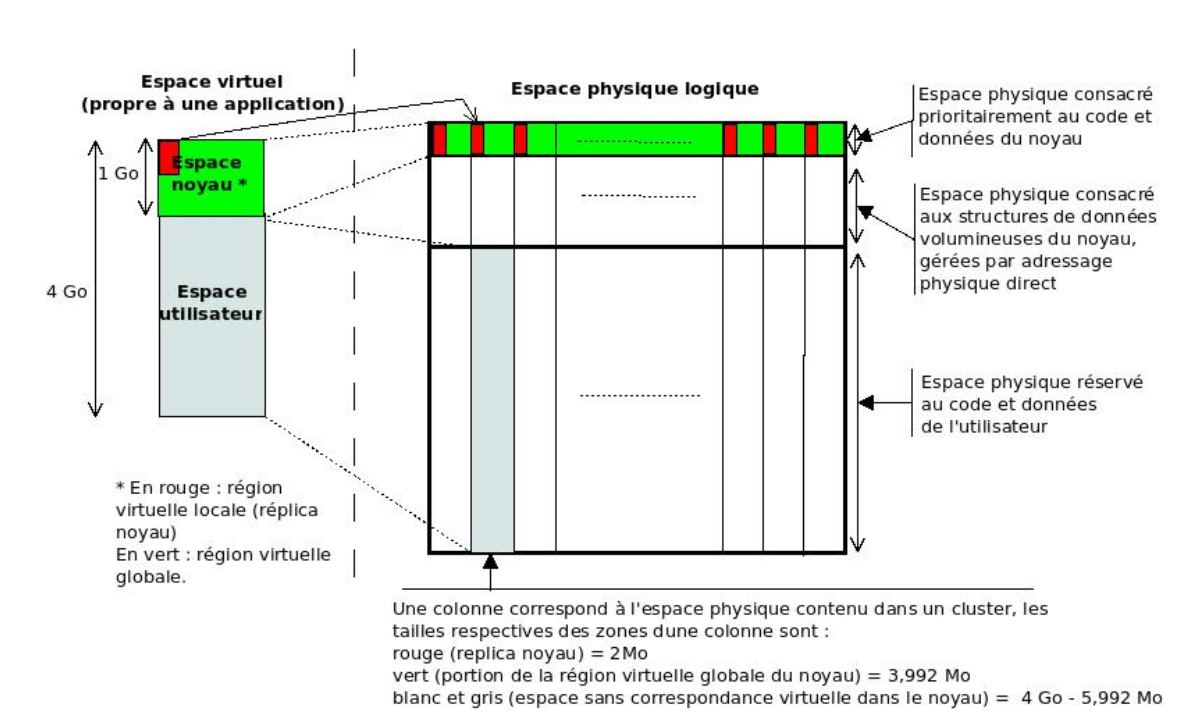
\includegraphics[scale=0.26]{decoupage}
          \caption{Mapping de l'espace virtuel noyau dans la version de François}
        \end{figure}
      \end{frame}

      \begin{frame}{\subsecname}
        \vspace{2cm}
      Problèmes:
        %\begin{paragraph}{test}
        \begin{itemize}
          \item L'espace virtuel du noyau est d'environ 4Mo par cluster \newline $\rightarrow$ pas
                assez
          \item Beaucoup trop compliqué $\rightarrow$ pas fini. 
          \item On supporte au maximum environ 72Go de RAM. \\
        \end{itemize}
      %\end{paragraph}
      \end{frame}

    \subsection{ALMOS 40 bits - nouvelle version}

      \begin{frame}{\subsecname}
        \begin{itemize}
          \item le noyau est entièrement en adressage physique
          \item chaque cluster exécute une instance du noyau de manière
            indépendante
        \end{itemize}
          \begin{columns}[T]
            \begin{column}[T]{5cm}
              \begin{exampleblock}{Avantages}
              \begin{itemize}
                \item le noyau gère 1To de mémoire (4Go par cluster, contre 4Mo)
                \item on laisse 4Go de mémoire virtuelle à l'utilisateur
                \item les caches TLB sont uniquement utilisés par les
                  applications de l'utilisateur
              \end{itemize}
            \end{exampleblock}
          \end{column}
          \begin{column}[T]{5cm}
            \begin{alertblock}{Inconvénient}
              \begin{itemize}
                \item le noyau ne peut plus accéder de manière directe à la
                  mémoire des autres clusters
              \end{itemize}
            \end{alertblock}
          \end{column}
        \end{columns}
      \end{frame}

  \section{Conclusion}

      \begin{frame}{\secname}
        \vspace{2cm}
        But du stage:
        \begin{itemize}   
          \item Implémenter un service de création et de migration distante de processus sans accès direct à
            la mémoire des clusters voisins
            \begin{itemize}
              \item[1-] D'abord sur des processus mono-thread pour définir les
                mécanismes à mettre en place et identifier les difficultés
              \item[2-] Puis on ajoutera le multi-threading
            \end{itemize}
          \item Ré-implémenter la DQDT pour le choix du placement des processus à leur
            création et pour l'équilibrage de charge
        \end{itemize}
      \end{frame}


  %\section{Travail à faire}

    %\subsection{}

      %\begin{frame}{\secname}
        %\begin{itemize}
          %\item 
        %\end{itemize}
      %\end{frame}


\end{document}
